%==============================================================================
%  Bachelor's Thesis Defense
%  Hybrid Post-Quantum Key Exchange for WireGuard (X25519 + ML-KEM-768)
%  Mihai-Cristian Farcas  --  UBB, 2026
%
%  Build:   tectonic presentation.tex
%  Notes:   uncomment the \setbeameroption line below to print speaker notes
%==============================================================================
\documentclass[aspectratio=169,11pt]{beamer}

% --- speaker notes (uncomment to interleave note pages) ----------------------
% \setbeameroption{show notes}

\usepackage{booktabs}
\usepackage{amsmath,amssymb}
\usepackage{tikz}
\usetikzlibrary{arrows.meta}

% figures live in the thesis tree; reuse them directly
\graphicspath{{../thesis/figures/}}

%--- look & feel --------------------------------------------------------------
\usetheme{default}
\setbeamertemplate{navigation symbols}{}

\definecolor{pqprimary}{HTML}{0C6E6E} % dark cyan
\definecolor{pqaccent}{HTML}{C0392B}  % red  (for "broken" / alerts)
\definecolor{pqgood}{HTML}{1E8449}    % green (for "holds" / good)
\definecolor{pqgray}{HTML}{555555}

\setbeamercolor{structure}{fg=pqprimary}
\setbeamercolor{title}{fg=pqprimary}
\setbeamercolor{frametitle}{fg=white,bg=pqprimary}
\setbeamercolor{alerted text}{fg=pqaccent}
\setbeamercolor{itemize item}{fg=pqprimary}
\setbeamercolor{itemize subitem}{fg=pqprimary}
\setbeamercolor{block title}{fg=white,bg=pqprimary}
\setbeamercolor{block body}{bg=pqprimary!6}

\setbeamerfont{frametitle}{series=\bfseries}
\setbeamerfont{title}{series=\bfseries}
\setbeamertemplate{itemize item}{\textbullet}
\setbeamertemplate{itemize subitem}{--}

% frametitle with a coloured bar (auto-height, so multi-line titles never clip)
\setbeamertemplate{frametitle}{%
  \nointerlineskip
  \begin{beamercolorbox}[wd=\paperwidth,sep=5pt,leftskip=0.25cm,rightskip=0.25cm]{frametitle}%
    \usebeamerfont{frametitle}\insertframetitle%
  \end{beamercolorbox}%
}

% minimal footline: short title  ........  frame number
\setbeamertemplate{footline}{%
  \leavevmode%
  \hbox{%
    \begin{beamercolorbox}[wd=.72\paperwidth,ht=2.4ex,dp=1ex,leftskip=.3cm]{author in head/foot}%
      \usebeamerfont{footline}\color{pqgray}\footnotesize Farca\c{s} -- Hybrid PQ Key Exchange for WireGuard%
    \end{beamercolorbox}%
    \begin{beamercolorbox}[wd=.28\paperwidth,ht=2.4ex,dp=1ex,rightskip=.3cm]{author in head/foot}%
      \hfill\usebeamerfont{footline}\color{pqgray}\footnotesize\insertframenumber\,/\,\inserttotalframenumber%
    \end{beamercolorbox}%
  }%
}

\newcommand{\sskem}{\ensuremath{ss_{\mathit{kem}}}}

%--- title metadata -----------------------------------------------------------
\title[Hybrid PQ Key Exchange for WireGuard]{Hybrid Post-Quantum Key Exchange for WireGuard}
\subtitle{Integrating ML-KEM into a Production Rust Userspace Implementation}
\author[M.-C. Farca\c{s}]{Mihai-Cristian Farca\c{s}}
\institute{Babe\c{s}--Bolyai University \\ Faculty of Mathematics and Computer Science}
\date{Bachelor's Thesis Defense \quad\textbar\quad June 2026}

\begin{document}

%==============================================================================
% 1 -- TITLE
%==============================================================================
{\setbeamertemplate{footline}{}
\begin{frame}[plain]
  \titlepage
  \vfill
  {\small\color{pqgray}Supervisor: Prof.\ Dr.\ Darabant Sergiu Adrian}
\end{frame}}
\note{One sentence: my thesis adds post-quantum protection to WireGuard's key
exchange by integrating NIST-standardised ML-KEM into BoringTun's handshake, and
measures what it costs. Then move on.}

%==============================================================================
% ROADMAP
%==============================================================================
\begin{frame}{Roadmap}
  \begin{enumerate}
    \item The problem -- why WireGuard needs post-quantum key exchange
    \item Two approaches -- PSK-slot baseline \& full hybrid
    \item The hybrid handshake (design)
    \item Implementation -- BoringTun and the \texttt{pq} feature
    \item Security analysis \& evaluation
    \item Conclusions
  \end{enumerate}
\end{frame}
\note{Fifteen seconds. Motivation, the two approaches, the hybrid design,
implementation, security and evaluation, conclusions. Don't dwell.}

%==============================================================================
% 2 -- MOTIVATION
%==============================================================================
\begin{frame}{Motivation: the quantum clock is already running}
  \begin{itemize}
    \item WireGuard's key exchange rests \alert{entirely on X25519}.
    \item Shor's algorithm breaks X25519 once a large quantum computer exists.
    \item \textbf{Harvest-now, decrypt-later:} adversaries can record encrypted
          traffic \emph{today} and decrypt it \emph{later}.
    \item[$\Rightarrow$] For long-lived secrets, migration is urgent \emph{now}.
  \end{itemize}
  \vfill
  \begin{block}{The standards landscape}
    NIST finalised \textbf{FIPS 203 (ML-KEM)} in Aug 2024 -- the standard for
    key exchange. Classical key exchange to be \textbf{deprecated by 2030},
    disallowed by 2035.
  \end{block}
\end{frame}
\note{WireGuard replaced IPsec/OpenVPN -- in the kernel, every OS, deployed by
Cloudflare, Mullvad, Tailscale. But all key agreement rests on X25519, which Shor
breaks. The threat is not future: harvest-now-decrypt-later means record now,
decrypt later. NIST has put dates on it and standardised ML-KEM.}

%==============================================================================
% 3 -- WHY WIREGUARD IS HARD
%==============================================================================
\begin{frame}{WireGuard: important, but hard to migrate}
  \begin{itemize}
    \item Fixed cipher suite, \textbf{no negotiation} -- a security feature
          (kills downgrade attacks)\ldots
    \item \ldots but \alert{no built-in way to swap the key-exchange algorithm}.
  \end{itemize}
  \vfill
  \begin{block}{Two natural handles for post-quantum augmentation}
    \begin{enumerate}
      \item The \textbf{PSK slot} -- a 256-bit symmetric key mixed into the
            handshake's key derivation.
      \item The \textbf{Noise IK handshake} itself -- embed a KEM alongside
            X25519 in every handshake.
    \end{enumerate}
  \end{block}
  \vfill
  \centering\small\color{pqgray} This thesis builds on \textbf{both}.
\end{frame}
\note{WireGuard is deliberately opinionated: one cipher suite, no negotiation.
That rigidity is why it avoided TLS/IPsec downgrade bugs, but it makes PQ
migration hard. Two handles: the existing PSK slot, and the Noise IK handshake
itself. I built both.}

%==============================================================================
% 4 -- RESEARCH QUESTION + TWO APPROACHES
%==============================================================================
\begin{frame}{Research question and two approaches}
  \begin{block}{Research question}
    Can WireGuard's handshake be extended with \textbf{hybrid post-quantum key
    exchange (X25519 + ML-KEM-768)} while preserving its security properties and
    staying viable on \textbf{resource-constrained hardware}?
  \end{block}
  \vfill
  \begin{columns}[T]
    \begin{column}{0.48\textwidth}
      \textbf{A. PSK-slot baseline}
      \begin{itemize}\small
        \item One-time ML-KEM exchange out-of-band $\to$ fill the PSK slot.
        \item \textbf{Zero} WireGuard changes; works with any client.
        \item The \emph{lower bound} on engineering effort -- a controlled
              comparison point.
      \end{itemize}
    \end{column}
    \begin{column}{0.48\textwidth}
      \textbf{B. Full hybrid \hfill\small\color{pqprimary}(the contribution)}
      \begin{itemize}\small
        \item ML-KEM-768 \emph{inside} the Noise IK handshake, every session.
        \item Fresh KEM keypair per handshake.
        \item Target: \textbf{BoringTun} (Cloudflare's production Rust userspace
              WireGuard).
      \end{itemize}
    \end{column}
  \end{columns}
  \vfill
  \centering\small\color{pqgray} To our knowledge, the first FIPS 203-compliant
  \emph{hybrid} WireGuard on a production codebase.
\end{frame}
\note{Slow down here -- this is the framing. RQ on the slide. Two attacks.
Approach A: minimal, out-of-band ML-KEM into the existing PSK slot, no protocol
change; built as a baseline to quantify what B buys. Approach B is the real
contribution: ML-KEM inside the handshake, fresh keys per session, on BoringTun
so it deploys in userspace.}

%==============================================================================
% 5 -- KEM vs DH + HYBRID IDEA
%==============================================================================
\begin{frame}{Just enough background: a KEM is not a Diffie--Hellman}
  \centering
  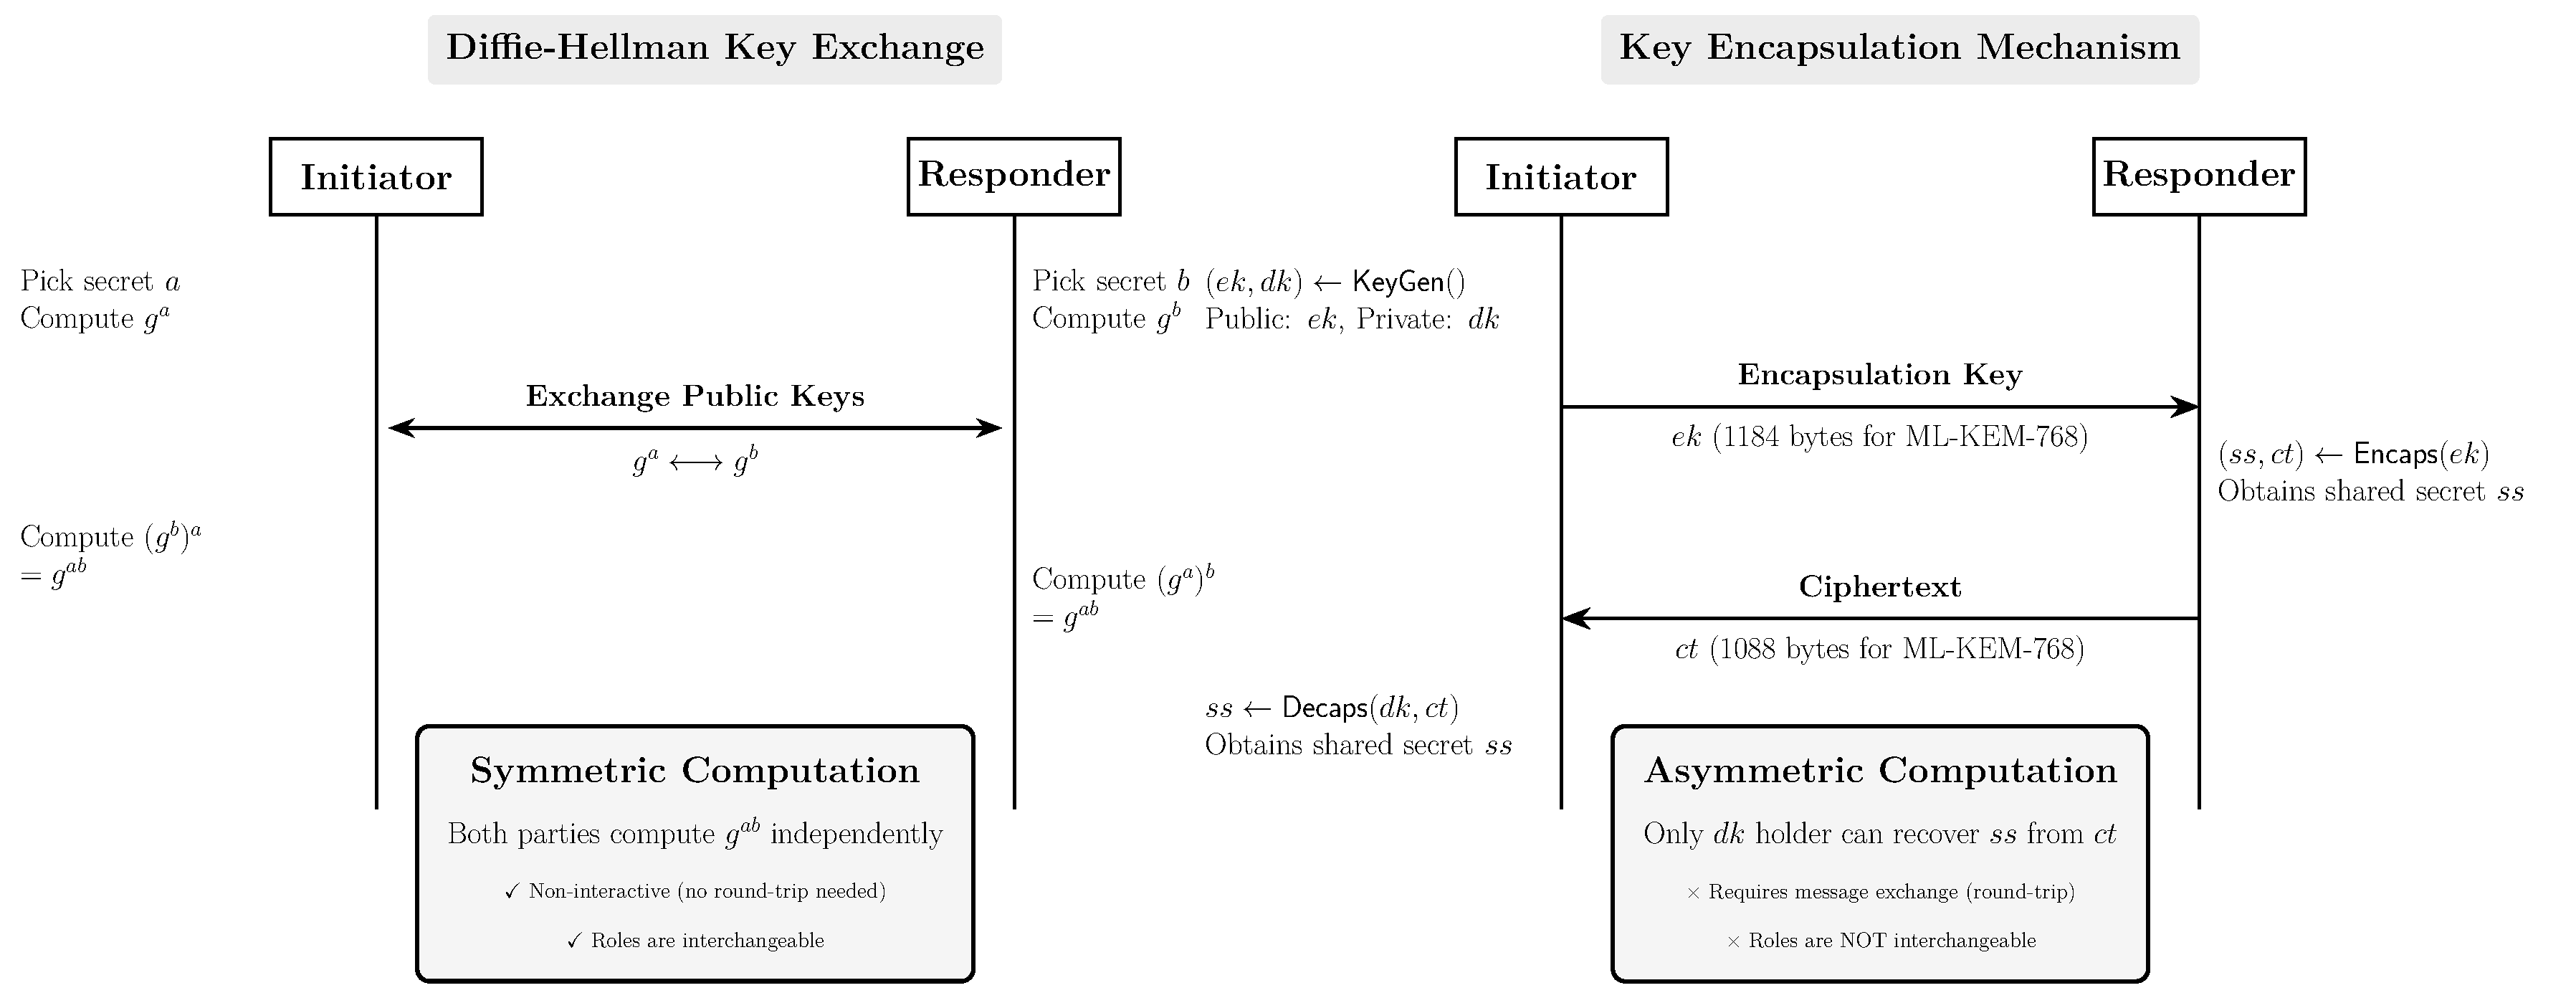
\includegraphics[width=\textwidth,height=0.6\textheight,keepaspectratio]{fig_kem_vs_dh}
  \vfill
  \begin{block}{Hybrid}
    \small X25519 is a symmetric DH; ML-KEM \emph{encapsulates / decapsulates}
    (asymmetric -- this shapes the handshake). The hybrid folds \emph{both}
    secrets together via concatenate-then-KDF (NIST SP 800-56C; the TLS 1.3
    pattern). \textbf{Secure if \emph{either} X25519 \emph{or} ML-KEM survives.}
  \end{block}
\end{frame}
\note{Mental-model shift, no lattice math. X25519 is a DH -- symmetric. ML-KEM is
a KEM -- one side encapsulates a secret under the other's key, ships a ciphertext.
That asymmetry shapes the handshake. Hybrid = fold both secrets in; the payoff is
the bold line: safe as long as one primitive holds. ML-KEM is young, so I hedge
with X25519.}

%==============================================================================
% 6 -- THE HYBRID HANDSHAKE (figure, near-full frame)
%==============================================================================
\begin{frame}{The hybrid handshake: ML-KEM rides the existing two messages}
  \begin{columns}[c]
    \begin{column}{0.66\textwidth}
      \centering
      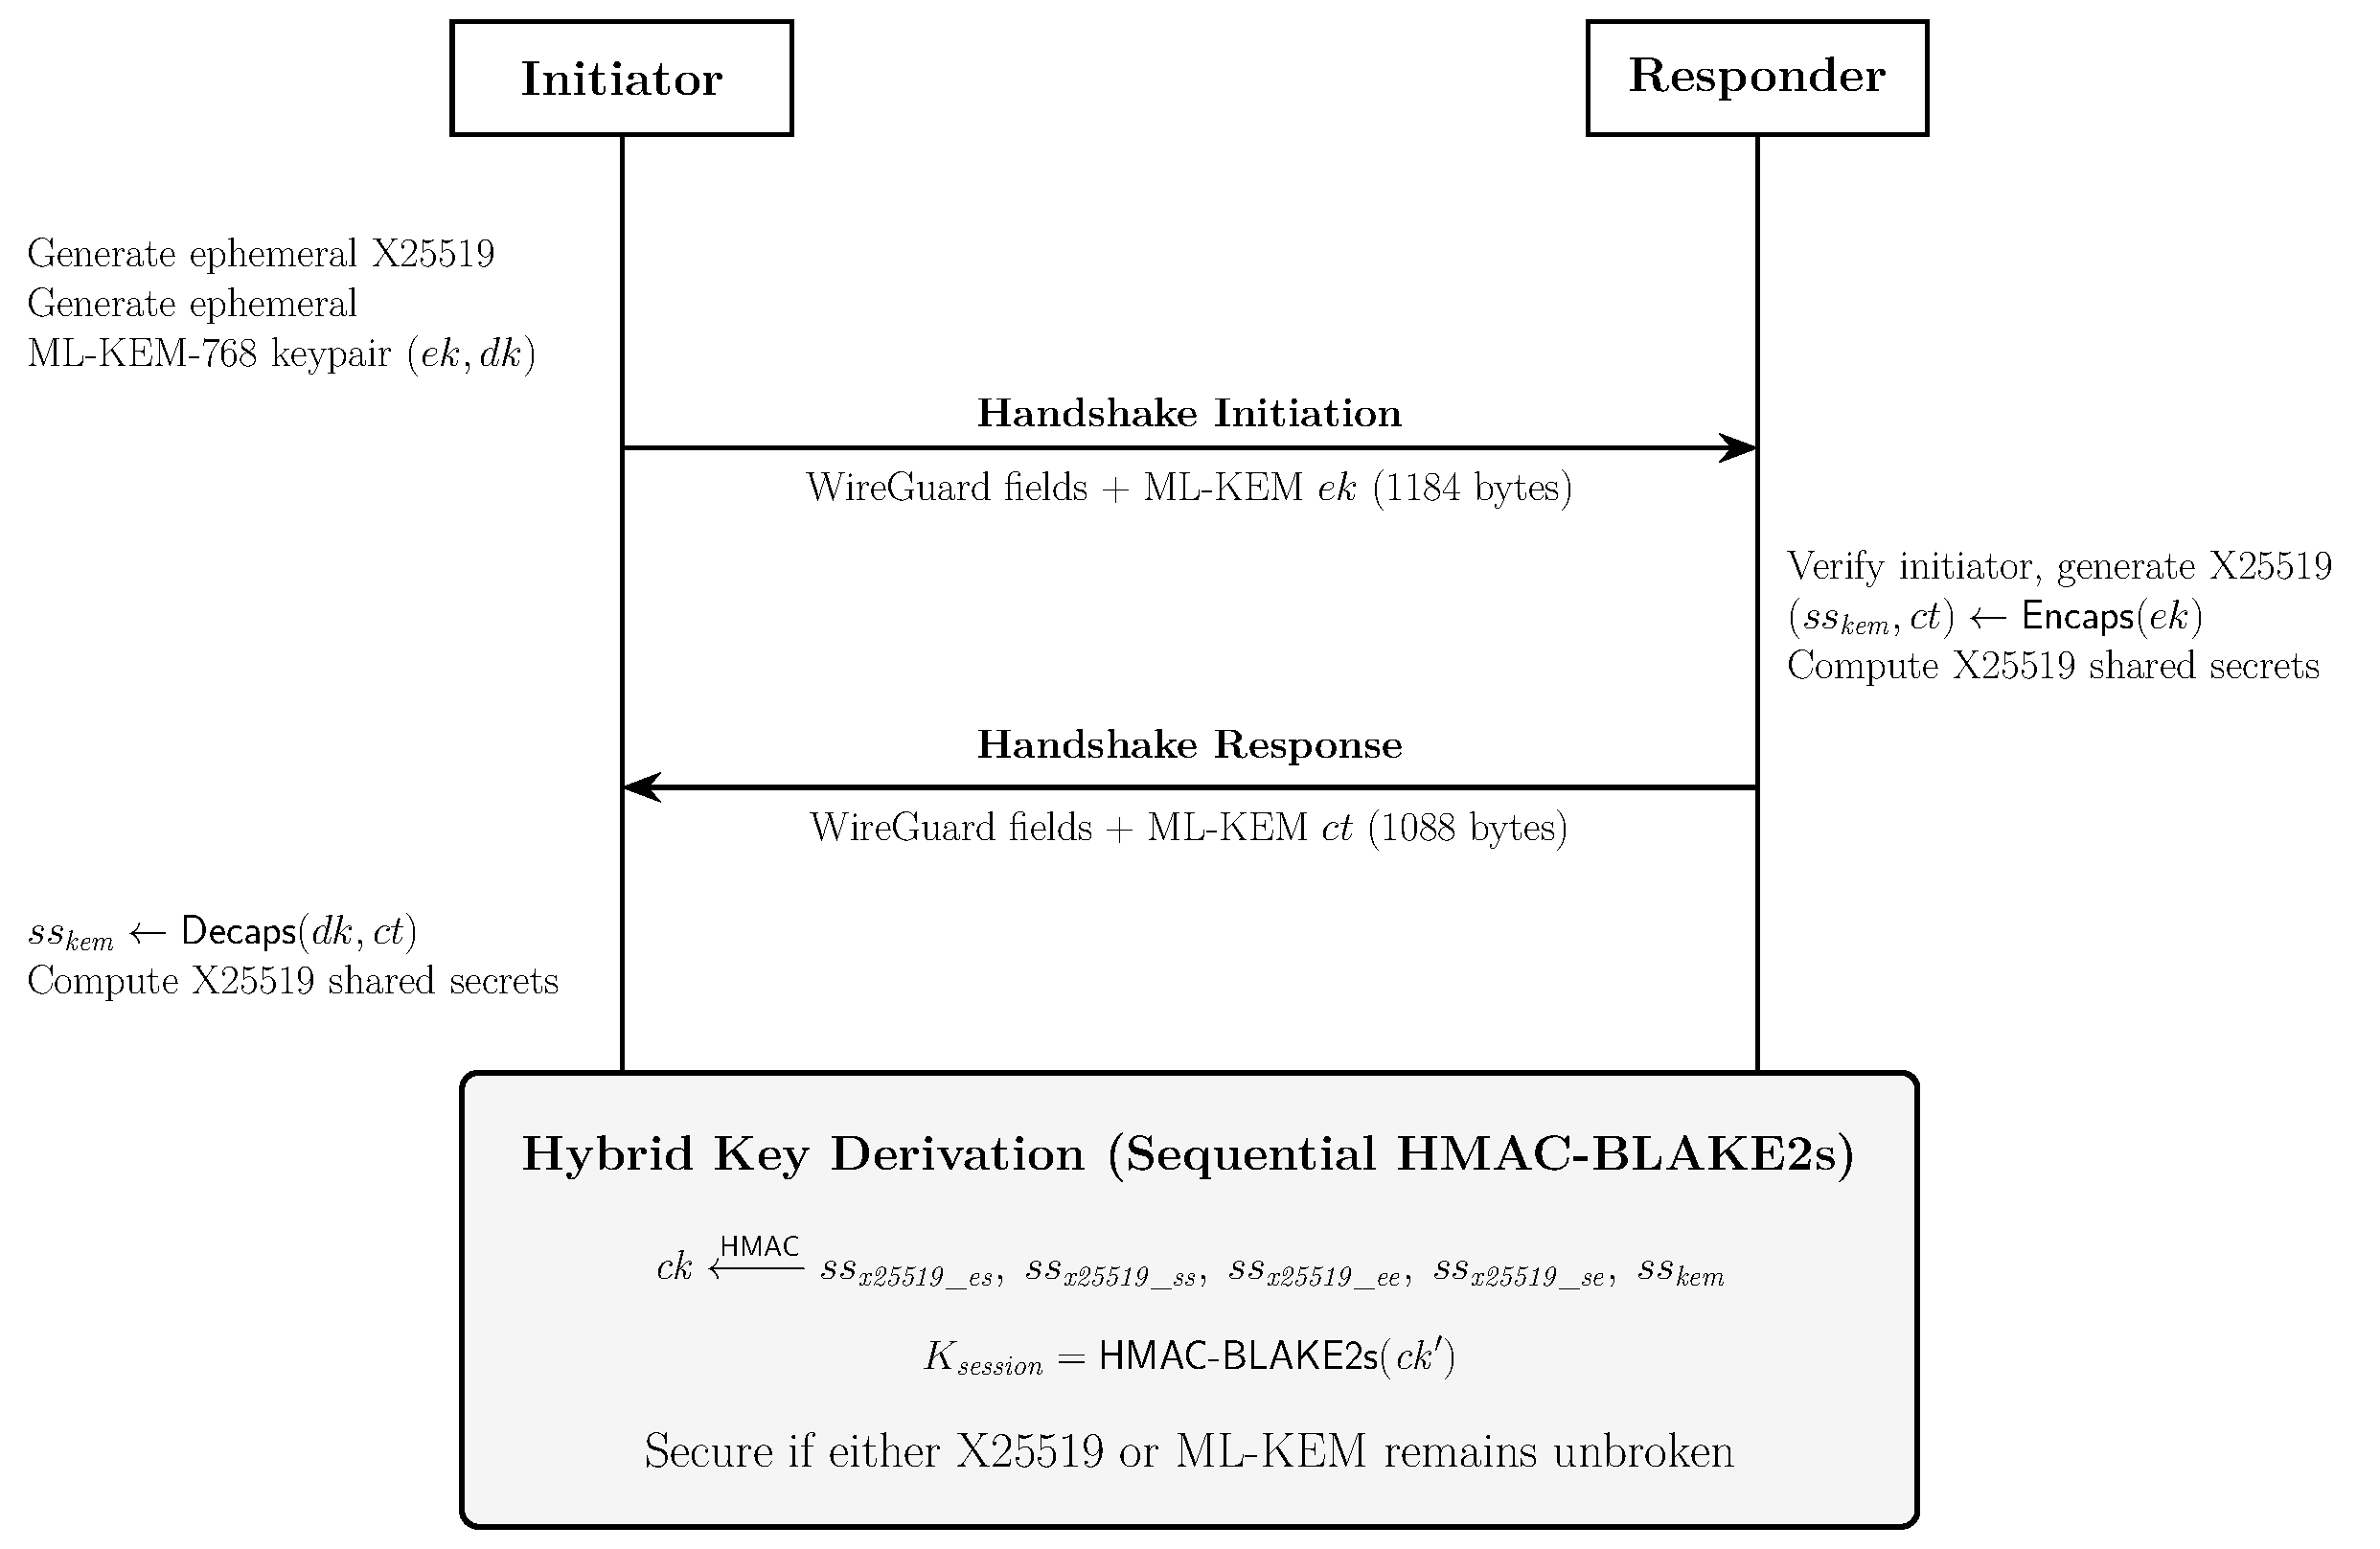
\includegraphics[width=\linewidth,height=0.82\textheight,keepaspectratio]{fig_hybrid_handshake}
    \end{column}
    \begin{column}{0.32\textwidth}
      \small
      \begin{itemize}
        \item \textbf{Msg 1:} WG fields \alert{+ ML-KEM $ek$ (1{,}184 B)}
        \item \textbf{Msg 2:} responder runs \textsf{Encaps} \alert{+ $ct$ (1{,}088 B)}
        \item Initiator \textsf{Decaps} $\to$ both share \sskem
      \end{itemize}
      \vspace{0.3em}
      \footnotesize\color{pqgray}
      No extra round trips. $ek$/$ct$ sit \emph{before} the MACs, so the
      anti-DoS cookie still covers the PQ payload.
    \end{column}
  \end{columns}
\end{frame}
\note{Core of the thesis -- walk the diagram. Fresh ML-KEM keypair per handshake;
ek in message one. Responder runs Encaps, returns ct in message two. Initiator
decapsulates -- same secret, no extra round trips. Design detail: ek/ct go before
the MAC fields, so MAC1/MAC2 cover them and the anti-DoS cookie extends to the PQ
payload for free.}

%==============================================================================
% 7 -- KEY DERIVATION + WHAT STAYS UNTOUCHED
%==============================================================================
\begin{frame}{Combining the secrets -- and what stays untouched}
  \begin{block}{One extra mixing step, using WireGuard's own KDF}
    After the four X25519 secrets are mixed in as usual, fold in \sskem:
    \[
      temp = \mathsf{HMAC\text{-}BLAKE2s}(ck,\ \sskem),\qquad
      ck' = \mathsf{HMAC\text{-}BLAKE2s}(temp,\ \mathtt{0x01})
    \]
    $ek$ and $ct$ are also bound into the transcript hash $h$.
  \end{block}
  \vfill
  \begin{itemize}
    \item \textbf{Reuses WireGuard's HMAC-BLAKE2s} -- no new HKDF/SHA-256
          introduced; keeps the security argument clean.
    \item \alert{Transport phase is byte-for-byte unchanged} -- ChaCha20-Poly1305
          untouched. \emph{This is why throughput is identical.}
  \end{itemize}
\end{frame}
\note{How the secrets combine: after the four X25519 results, one extra
HMAC-BLAKE2s step folds in the KEM secret; ek and ct bound into the transcript
hash. Two points: I reuse WireGuard's own KDF (clean security argument), and I
touch only the handshake -- the ChaCha20-Poly1305 data plane is unchanged, which
is why throughput is identical later.}

%==============================================================================
% 8 -- IMPLEMENTATION
%==============================================================================
\begin{frame}{Implementation}
  \begin{itemize}
    \item All PQ code behind a Cargo \texttt{pq} feature flag $\Rightarrow$
          \textbf{a vanilla build is byte-for-byte identical to upstream}.
    \item \texttt{ml-kem} crate (RustCrypto): pure-Rust, \texttt{no\_std},
          NIST KAT-tested $\Rightarrow$ runs on the Pi, \textbf{no C FFI}.
    \item New message types \textbf{5} (PQ init) and \textbf{6} (PQ response);
          parser dispatches on type+size; a vanilla build cleanly rejects them
          (\texttt{InvalidPacket}).
    \item Memory-safe Rust; minimal carried state (initiator keeps only $dk$,
          responder only $ek$).
  \end{itemize}
  \vfill
  \begin{block}{Testing}
    Extended BoringTun's own Criterion benchmarks and \texttt{noise::tests}:
    full PQ handshake, end-to-end transport, ML-KEM/PSK orthogonality, and
    vanilla-rejects-PQ.
  \end{block}
\end{frame}
\note{Everything PQ sits behind the pq feature -- so a build without it is
byte-for-byte upstream BoringTun (that's how I get a clean baseline). ML-KEM via
the pure-Rust RustCrypto crate, KAT-tested, no C FFI, runs on the Pi. Two new
message types, 5 and 6; vanilla rejects them gracefully. Extended BoringTun's own
test suite to cover the PQ paths.}

%==============================================================================
% 9 -- SECURITY
%==============================================================================
\begin{frame}{Security analysis}
  \begin{block}{Hybrid-secure}
    The session key is indistinguishable from random if \textbf{X25519
    \emph{or} ML-KEM} is secure (concatenate-then-KDF; HMAC-BLAKE2s as a PRF).
  \end{block}
  \begin{itemize}
    \item \textcolor{pqgood}{\textbf{Post-quantum forward secrecy:}} fresh ML-KEM
          keypair \emph{per handshake} $\Rightarrow$ past sessions stay safe even
          if X25519 later falls.
          \\ \small\color{pqgray} The PSK-slot baseline \textbf{cannot} match
          this: a static PSK, one compromise exposes many sessions.
    \item \textcolor{pqaccent}{\textbf{Authentication stays classical}} (X25519
          static keys) -- \emph{deliberate}: it cannot be broken
          \emph{retroactively}, and NIST prioritises key-exchange migration over
          signatures. ML-DSA is future work.
  \end{itemize}
\end{frame}
\note{Three claims. Hybrid security: both secrets feed a PRF-based KDF, so the key
looks random if either holds -- informal reduction via the concatenation
combiner. The key win over the baseline: fresh KEM keypair per handshake gives
post-quantum forward secrecy; the PSK-slot reuses one static PSK, so one
compromise exposes everything. Honest limitation: authentication is still
classical X25519 -- deliberate, can't be forged retroactively, NIST says migrate
KEX first.}

%==============================================================================
% 10 -- EVALUATION: LATENCY
%==============================================================================
\begin{frame}{Evaluation -- handshake latency (Criterion, 95\% CI)}
  \begin{table}
    \centering\small
    \begin{tabular}{@{}lcc@{}}
      \toprule
      \textbf{Configuration} & \textbf{Apple M4} & \textbf{Raspberry Pi 5} \\
      \midrule
      Vanilla   & 150.8\,$\mu$s & 1312\,$\mu$s \\
      PSK-slot  & 151.0\,$\mu$s & 1312\,$\mu$s \\
      \textbf{Hybrid} & \textbf{247.3\,$\mu$s (+64\%)} & \textbf{1643\,$\mu$s (+25\%)} \\
      \bottomrule
    \end{tabular}
  \end{table}
  \vfill
  \begin{itemize}\small
    \item Overhead $\approx$ the three ML-KEM ops ($\approx$73\,$\mu$s M4 /
          $\approx$280\,$\mu$s Pi); the rest is bigger buffers + an extra hash pass.
    \item \alert{It is 64\% of a \emph{sub-millisecond, crypto-only} cost} --
          over a real link, RTT dominates and the data plane is untouched.
    \item \textbf{Surprise:} on the Pi, one X25519 DH (193\,$\mu$s) is
          \emph{slower} than any ML-KEM op -- \texttt{x25519-dalek} lacks NEON;
          ML-KEM's NTT maps well to the integer pipeline.
  \end{itemize}
\end{frame}
\note{Criterion microbenchmarks, 500 samples, bootstrapped CIs, on M4 and Pi 5 --
two ends of the ARM64 spectrum. Hybrid adds 64% on M4, 25% on Pi -- but it's 64%
of a sub-millisecond crypto-only cost. PSK-slot is indistinguishable from vanilla,
as expected. The memorable finding: on the Pi a single X25519 DH is slower than
any ML-KEM op, because x25519-dalek doesn't use NEON while ML-KEM's NTT maps onto
the integer pipeline. Deliver this one with a bit of "this surprised me".}

%==============================================================================
% 11 -- EVALUATION: SIZE / THROUGHPUT / FOOTPRINT
%==============================================================================
\begin{frame}{Evaluation -- size, throughput, footprint}
  \begin{itemize}
    \item \textbf{Packet size is the real cost:} handshake grows
          \textbf{240 B $\to$ 2{,}512 B} (+2{,}272 B). Both messages still fit a
          1{,}500 B Ethernet MTU \alert{in a single datagram} -- confirmed over
          real Wi-Fi, no fragmentation.
    \item \textbf{Throughput unchanged:} $\sim$470 Mbps loopback, $\sim$80--85
          Mbps cross-device; vanilla vs hybrid CIs overlap (same
          ChaCha20-Poly1305 data plane).
    \item \textbf{Footprint negligible:} binary \textbf{+65 KiB} (+5.7\%), peak
          RSS \textbf{+0.16 MiB} -- a non-issue even on the Pi.
  \end{itemize}
  \vfill
  \centering\small\color{pqgray}
  The cost of the hybrid is \emph{size}, not time -- and the size still fits.
\end{frame}
\note{Three quick results. The real cost is size: handshake grows tenfold to
~2.5 KB, but both messages fit a 1500-byte frame as a single datagram -- verified
over real Wi-Fi. Throughput identical (same data plane) -- this table is a
correctness check. Footprint: ~65 KiB code, fraction of a MiB RAM. Tagline: the
cost is size, not time, and the size still fits.}

%==============================================================================
% 12 -- CONCLUSIONS
%==============================================================================
\begin{frame}{Conclusions}
  \begin{block}{Contributions}
    \begin{enumerate}\small
      \item First FIPS 203-compliant \emph{hybrid} WireGuard on a production Rust
            codebase.
      \item A PSK-slot baseline as a controlled comparison point.
      \item A hybrid Noise IK handshake with \emph{post-quantum forward secrecy}.
      \item Evaluation across two ARM tiers (Apple M4, Raspberry Pi 5).
    \end{enumerate}
  \end{block}
  \vfill
  \textbf{Bottom line:} hybrid PQ WireGuard is \textbf{practical today} --
  NIST-aligned, userspace-deployable, sub-millisecond overhead, data plane
  untouched.
  \vfill
  \small\color{pqgray}\textbf{Future work:} MTU strategies (segmentation / PMTUD);
  ML-DSA authentication; a formal proof; ML-KEM parameter agility.
\end{frame}
\note{Four contributions on the slide. Takeaway: hybrid PQ WireGuard is practical
today -- NIST standards, userspace, sub-ms overhead, data plane untouched. Open
problems: MTU on hostile paths, PQ authentication via ML-DSA, a formal proof
(Hybrid-WireGuard is the template).}

%==============================================================================
% 13 -- THANK YOU
%==============================================================================
{\setbeamertemplate{footline}{}
\begin{frame}[plain]
  \centering
  \vfill
  {\usebeamerfont{title}\color{pqprimary}\Large Thank you.}\\[1.2em]
  {\large Questions?}\\[2em]
  {\small\color{pqgray} Mihai-Cristian Farca\c{s} \quad\textbar\quad
   Supervisor: Prof.\ Dr.\ Darabant Sergiu Adrian}
  \vfill
\end{frame}}

%==============================================================================
% BACKUP SLIDES
%==============================================================================
\appendix

\begin{frame}{Backup -- per-primitive microbenchmarks (Criterion)}
  \begin{table}
    \centering\small
    \begin{tabular}{@{}lcc@{}}
      \toprule
      \textbf{Operation} & \textbf{Apple M4} & \textbf{Raspberry Pi 5} \\
      \midrule
      ML-KEM-768 KeyGen & 24.13\,$\mu$s & \phantom{0}81.66\,$\mu$s \\
      ML-KEM-768 Encaps & 20.82\,$\mu$s & \phantom{0}82.77\,$\mu$s \\
      ML-KEM-768 Decaps & 28.03\,$\mu$s & 115.15\,$\mu$s \\
      \midrule
      X25519 KeyGen     & \phantom{0}8.77\,$\mu$s & \phantom{0}58.00\,$\mu$s \\
      X25519 DH         & 20.39\,$\mu$s & 192.81\,$\mu$s \\
      \bottomrule
    \end{tabular}
  \end{table}
  \centering\small\color{pqgray}
  On the Pi, a single X25519 DH costs more than any ML-KEM operation.
\end{frame}

\begin{frame}{Backup -- the PSK-slot baseline}
  \centering
  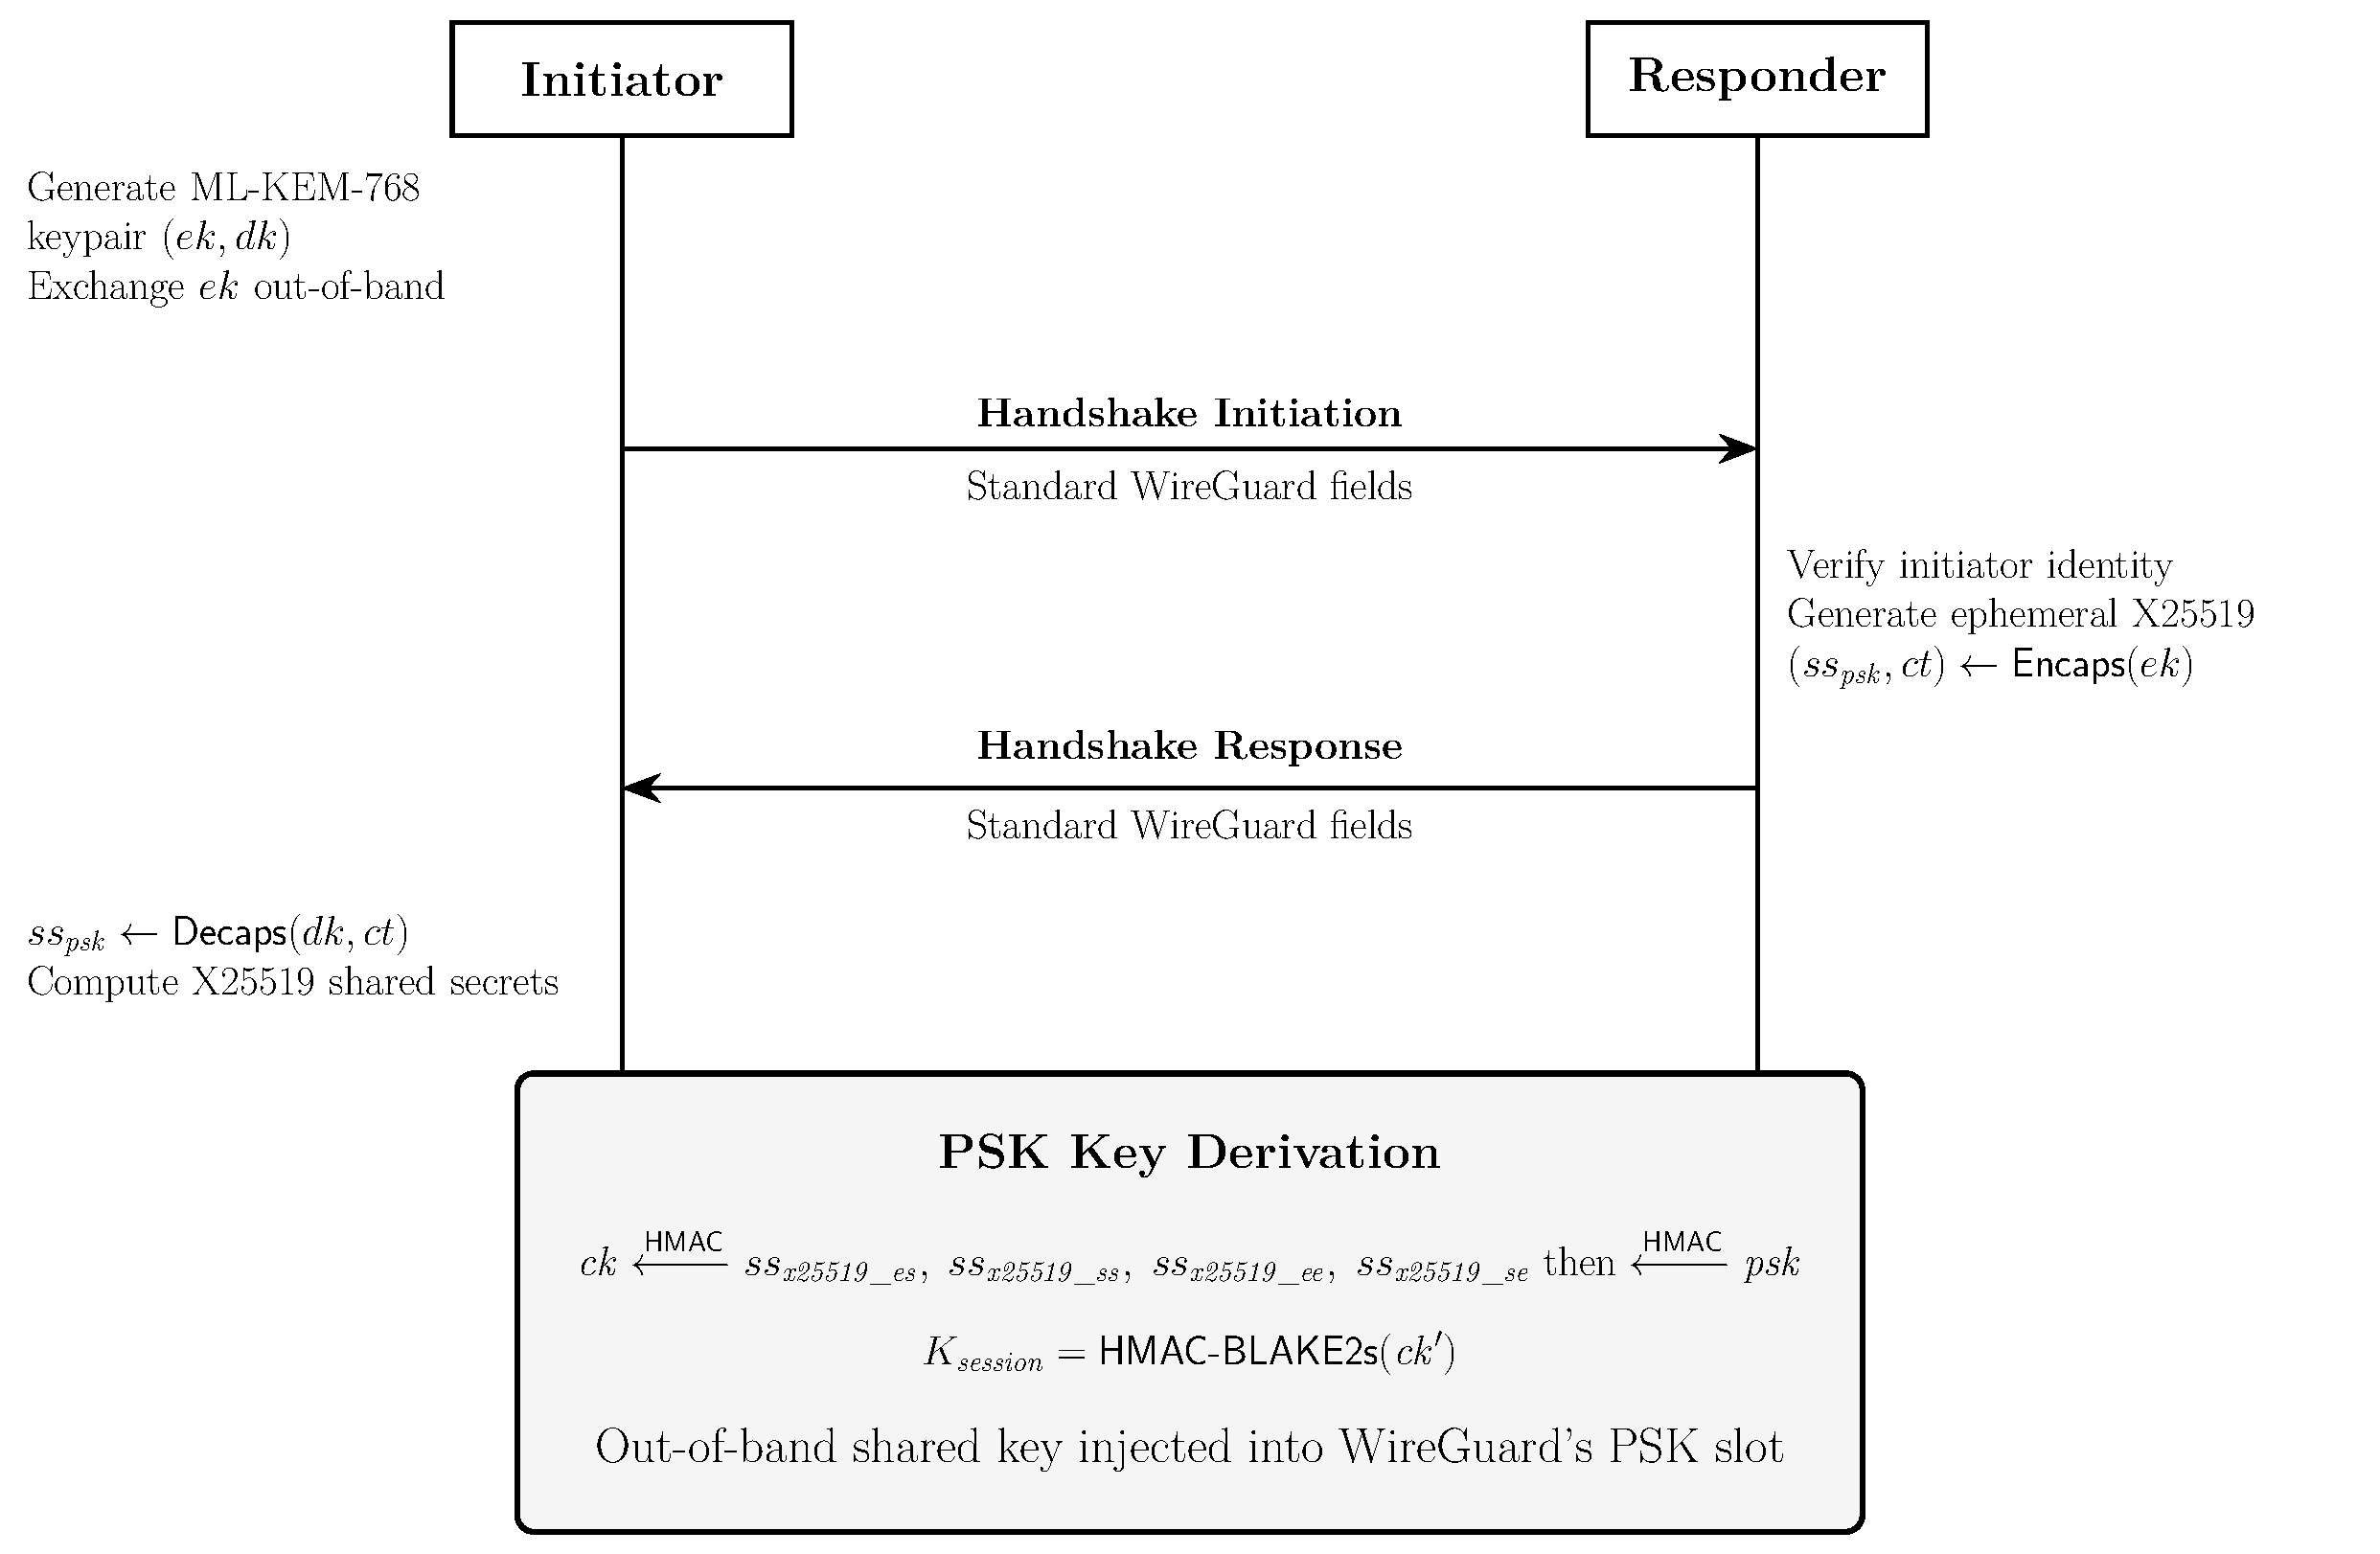
\includegraphics[width=\textwidth,height=0.85\textheight,keepaspectratio]{fig_psk_handshake}
\end{frame}

\begin{frame}{Backup -- MTU \& interoperability}
  \begin{itemize}
    \item Hybrid initiation 1{,}332 B; fragmentation only on paths below
          $\sim$1{,}360 B (e.g.\ IPv6's 1{,}280 B minimum).
    \item \textbf{Lowering the WireGuard MTU does \emph{not} help} -- that shrinks
          data packets, not the fixed-size handshake. The fix must live in the
          handshake (app-level segmentation / PMTUD -- future work).
    \item Interop: a vanilla peer drops PQ types 5/6 at dispatch
          (\texttt{InvalidPacket}); no crash, but no auto-fallback -- both peers
          must be hybrid-capable. Capability negotiation is engineering, not
          fundamental.
  \end{itemize}
\end{frame}

\begin{frame}{Backup -- why ML-KEM-768, why hybrid}
  \begin{itemize}
    \item \textbf{ML-KEM-768:} NIST Level 3 ($\sim$AES-192); the general-purpose
          default recommended by NIST/IETF; balances size vs security.
    \item \textbf{Hybrid, not pure-PQ:} the MLWE assumption is young; pairing with
          X25519 means a future lattice break still leaves sessions protected.
          NIST and IETF recommend hybrid for the transition.
    \item \textbf{vs related work:} PQ-WireGuard is pure-PQ on prototypes with
          non-standard KEMs; Rosenpass/ExpressVPN carry PQ secrets through the PSK
          slot. This work modifies the Noise handshake directly, on production
          code, with standardised ML-KEM -- complementary to the formal
          Hybrid-WireGuard proof (Lafourcade et al.).
  \end{itemize}
\end{frame}

\end{document}
